\documentclass[a4paper,11pt]{article}
\usepackage[frenchb]{babel}
\usepackage[T1]{fontenc}
\usepackage[utf8]{inputenc}
\usepackage{lmodern}
\usepackage{microtype}

\usepackage{array,multirow,makecell}
\setcellgapes{1pt}
\makegapedcells
\usepackage{caption}
\usepackage{adjustbox}

\usepackage{amsmath,amssymb,bm,upgreek,stmaryrd,mathrsfs,systeme}

\usepackage{graphicx}

\usepackage{geometry}
\geometry{hmargin=3cm,vmargin=2cm}

\usepackage{hyperref}

\title{Données utilisées et sources}

\begin{document}
\maketitle

Constante de Stefan-Boltzmann:

\[\sigma = \frac{2\pi^{5}k^{4}}{15h^{3}c^{2}} \approx 5,670374419 \times 10^{-8} W \cdot m^{-2} \cdot K ^{-4} \] \\

Température du soleil $T_s$: \\

On remarque sur le graphe précédent qu'il existe un pic de $u(\lambda)$ et que selon la température $T$, le pic n'est pas à la même longueur d'onde. \\

\begin{adjustbox}{center}
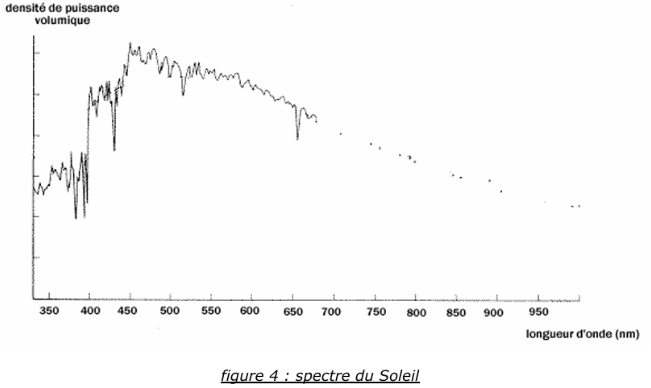
\includegraphics[scale=0.5]{densite_puissance}
\end{adjustbox}
\begin{figure}[h]
  \centering
  \caption{Densité de puissance}
\end{figure}

La loi de déplacement de Wien donne la longueur d'onde $\lambda_m$ pour laquelle on a le maximum de puissance en fonction de la température $T$. $h$ est la constante de Planck et $c$ la célérité de la lumière.

\[ \lambda_m = \dfrac{hc}{4,96kT} = \dfrac{2,898 \cdot 10^{-3}}{T} \]

Avec $\lambda_{(Soleil)} = 500 nm$

En isolant $T$, on fait l'application numérique de la température du Soleil:

\[ T_s= \dfrac{2.89 \times 10^{-3}}{500 \times 10^{-9}} = 5780 K \]



Distance Terre-Soleil $d_{T-S}$ :

L' unité astronomique (AU) est une unité de longueur définie pour être exactement égale à 149 597 870 700 m. Historiquement, l'unité astronomique était conçue comme la distance moyenne Terre-Soleil (la moyenne de l'aphélie et du périhélie de la Terre ), avant sa redéfinition moderne en 2012. 

On a donc $d_{T-S} = 149~597~870~700~m$.

Le détail pour déterminer cette valeur est long et complexe (il passer par le calcul d'arc de cercles), pour plus d'informations, aller à : \url{https://en.wikipedia.org/wiki/Astronomical_unit}.

Voici le lien d'un document expliquant le calcul de la température du Soleil : \url{https://perso.ensta-paris.fr/~perez/Media/Ressources/papiers/Temp-Soleil.pdf}.

Rayon de la Terre $R_T$:
Rayon terrestre est la distance entre le centre de la Terre et un point situé à sa surface ou à proximité. En se rapprochant de la figure de la Terre par un sphéroïde terrestre , le rayon varie d'un maximum de près de 6 378 km à un minimum de près de 6 357 km.

L'Union géodésique et géophysique internationale (UGGI) définit le rayon moyen $R_T$ à partir du rayon équatorial $a$ (demi-grand axe) et du rayon polaire $b$ (demi-petit axe) par la relation (\url{https://en.wikipedia.org/wiki/Earth_radius}) :

\[R_T = \dfrac {2a+b}{3}\]

Pour la considération de l'effet de serre, nous avons utilisé les ressources de deux sites : \url{https://vademecum.brandenberger.eu/pdf/klima/legendre_calcul_co2.pdf} et \url{https://planet-terre.ens-lyon.fr/ressource/principes-effet-serre.xml}.









\end{document}